\documentclass[12pt,twoside]{article}
\usepackage{jmlda}
\usepackage{url}
\usepackage{hyperref}
\usepackage{graphicx}
\usepackage[english]{babel}
\usepackage[T2A]{fontenc}

\makeatletter
\bibliographystyle{unsrt}
\renewcommand{\@biblabel}[1]{#1.}
\renewcommand{\figurename}{Fig.}
\renewcommand{\contentsname}{Table of Contents}
\renewcommand{\thesubfigure}{\alph{subfigure}}

\makeatother
\pgfplotsset{compat=1.18} 
%\NOREVIEWERNOTES
\title
    [Quasiperiodic time signals classification] 
    % Краткое название; не нужно, если полное название влезает в~колонтитул
    {Quasiperiodic time signals classification with spherical harmonics}
\author
    {Tikhonov~D.\,M.$^1$, Strijov~V.\,V.$^2$} % основной список авторов, выводимый в оглавление
    %\thanks
    %{Работа выполнена при финансовой поддержке РФФИ, проект \No\,00-00-00000.}
\email
   {tihonov.dm@phystech.edu;  strijov@ccas.ru}
\organization
{$^1$Moscow Institute of Physics and Technology (National Research University)\\
$^2$Computing Center im. A.A. Dorodnitsyn RAS}
%\thanks
%	{ }
\abstract
{\textbf{Abstract}: The problem of constructing a model of approximation and classification of quasi-periodic signals is solved.
The least \emph{structural complexity} is required.
\emph{Structural complexity}~---~is the number of a model parameters.
The time series is vectorized using the delay method to constract a phase space.
A subspace is chosen for a reduction of the complexity of the model in the phase space.
The phase trajectory in the resulting subspace is approximated by a linear combination of the spherical harmonics.
The obtained coefficients are used as a feature description.
The computational experiment was carried out on measurements of the accelerometer of a mobile device with three classes of human movements.

\bigskip
\textbf{Key words}: \emph{time series, approximation, classification, phase space, spherical harmonics}.}

\newcommand{\nsymbol}[2]{\medskip\hangindent=\parindent\hangafter=1\noindent $#1$ --- #2\par}
\newcommand{\nsymbolp}[3]{\nsymbol{#1}{#2 \dotfill\pageref{#3}}}

\newcommand{\hookuparrow}{\mathrel{\rotatebox[origin=t]{270}{$\hookleftarrow$}}}
\newcommand{\hookdownarrow}{\mathrel{\rotatebox[origin=t]{90}{$\hookleftarrow$}}}

\begin{document}
\maketitle

\section{Introduction}
The work is devoted to the classification of quasi-periodic time series.
Examples of such series are accelerometer and gyroscope readings during repetitive physical activity, electrocardiogram.

The classic approach is to use the nearest neighbor method in  combinations with various distance functions~\cite{Bagnall_2017}, or an ensemble of different types of discriminative models on various feature spaces~\cite{Hills_2014, Bostrom2017, Kate_2015}.
These approaches have a common property: a data transformation stage, in which the time series are transformed into a new feature space, for example, using the transformation shapelet ~\cite{ Hills_2014, Bostrom2017} or the DTW~\cite{Kate_2015} functions.
Another wide class of approaches to the solution~---~is various neural networks on the original time series~\cite{WANG_2019}, for example, the convolution neural networks.
Methods that combine the approach of generating features and direct use of time series are based on the method of delays and a classification of the obtained vector representations~\cite{Frank_2010}.
This work is the closest approach to the solution described in this paper and an alternative approach for comparison.

This paper proposes a time series classification model based on the spherical harmonic approximation model on the surface of a sphere.
For this purpose a transition to the space of phase trajectories or trajectory space is made.
The transition is carried out using the delay method~\cite{LAI19961}.
The delay method is used in the analysis of non-stationary time series.
For example, in the method of singular spectral analysis~\cite{Golyandina2002}, the decompositions into components and the prediction are based on the trajectory matrix.
It allows to move from a scalar time series to a multidimensional representation.
The delay method is also widely used in the analysis of nonlinear dynamical systems~\cite{Takens1981, LAI19961}.

The excessive dimension of the trajectory space ~\cite{Golyandina2002, Motrenko2015,Usmanova2020} leads to the instability of the models under study and an excessively complex description of the time series.
It is proposed to use the principal component method~\cite{Ezukwoke2019, Scholkopf1998} for dimensionality reduction of the phase space.

The phase trajectory is projected onto the $p$-dimensional unit sphere in the chosen low-dimensional phase subspace.
The function on the sphere surface is proposed to approximate by a linear combination of the spherical harmonics.
The obtained coefficients are further used as an feature description in the classification problem.


\begin{otherlanguage}{english}
\begin{figure}[H]
\centering
%   \subfloat[$s(t) = 2cos(2\pi\nu_1t + \varphi_1) + cos(2\pi\nu_2t + \varphi_2) + \varepsilon$]
  {\includegraphics[width=0.3\textwidth]{figs/synthetic_example.eps}}
%   \subfloat[Фазовая траектория (PCA)]
  {\includegraphics[width=0.35\textwidth]{figs/synthetic_trajectory.eps}}\\
\caption{Left: time series segment, right: phase trajectory.}
\label{fg:initial_traj}
\end{figure}
\end{otherlanguage}

Time series segment and its phase trajectory into a three-dimensional space are shown on Fig.~\ref{fg:initial_traj}.
The phase trajectory was obtained using the delays embedding method  and the principal components analysis method over the delay matrix.

%%%%%%%%%%%%%%%%%%%%%%%%%%%%%%%%%%%%%%%%%%%%%%%%%%%%%%%%%%%%%%%%%%%%%%%%%%%%%
\section{Spherical harmonics classification problem statement}

Let $\mathbf{S}$ is a set of time series, $\mathbf{Z}$ is a set of class numbers.
It is required to construct a mapping over finite sample $\mathbf{S}^{b} = \{(\mathbf{s}_1, y_1),\dots,(\mathbf{s}_{b}, y_{b}) \}$ , where $\mathbf{s}=[s_1,...,s_N]$ --- a time series, $b$ ---   a number of objects in the sample

\begin{equation}
y*:\mathbf{S} \xrightarrow{} \mathbf{Z}.
\label{eq:y*}
\end{equation}

A trajectory matrix is constructed with the existing time series $\mathbf{s}$

\begin{equation*}
    \mathbf{H}_{s}^{n} = 
    \begin{bmatrix} 
    	s_{1} & s_{2} & \ldots &s_{n-1} &s_{n}\\
    	s_{2} & s_{3} & \ldots &s_{n} &s_{n+1}\\
    	\vdots& \vdots & \ddots & \vdots & \vdots\\
    	s_{N-n+1} & s_{N-n+2} &\ldots&s_{N-1} &s_{N}\\
    \end{bmatrix} = 
	\begin{bmatrix} 
      	\mathbf{s}_{1}\\
      	\mathbf{s}_{2}\\
      	\vdots\\
      	\mathbf{s}_{m}\\
   \end{bmatrix},
   \quad
   m = N-n+1,
\label{eq:hankel_matrix}
\end{equation*}
where $N$~---~length of the time series, $n$~---~window size, not less than the estimated period, $\mathbf{s}_t=[s_{t},s_{t+1},\ldots,s_{t+n-1}] \in \mathbb{H}_{s} \subseteq \mathbb{R}^{n}$ --- vectors, forming the phase trajectory of the series $\mathbf{s}$.

The dimension of the trajectory space $\mathbb{H}_{s}^{n}$ is exx.
It is proposed to reduce the dimension of $\mathbb{H}_{s}^{n} \xrightarrow{} \mathbb{H}_{x}^{p}$ using the principal component method for $p \ll n $:

Размерность траекторного пространства $\mathbb{H}_{s}^{n}$ избыточна.
Предлагается снижать размерность $\mathbb{H}_{s}^{n} \xrightarrow{} \mathbb{H}_{x}^{p}$ с помощью метода главных компонент при $p \ll n $:
\begin{equation}
\mathbf{H}_{x}^{p} = \mathbf{H}_{s}^{n}\mathbf{U} =
\begin{bmatrix} 
  	\mathbf{x}_{1}\\
  	\mathbf{x}_{2}\\
  	\vdots\\
  	\mathbf{x}_{m}\\
\end{bmatrix},
\quad
\mathbf{x}_{t} \in \mathbb{R}^{p},
\quad
t \in [1,m]
\label{eq:PCA}
\end{equation}
where $\mathbf{U}$ is the transformation matrix of the principal component analysis method with the number of components equal to $p$ corresponding to the largest eigenvalues.

In the resulting subspace, the phase trajectory is translated from Cartesian to spherical coordinates $\mathbb{H}_{x}^{p} \xrightarrow{} \mathbb{S}_{r}^{p}$:
\[
    \phi: \mathbf{x} \xrightarrow{} \mathbf{r} = [r,\alpha_{p-1},\dots,\alpha_1],
    \quad
    \mathbf{a} = [\alpha_{p-1},\dots,\alpha_1],
    \quad
    \mathbf{S}_{r}^{p} = \phi(\mathbf{H}_{x}^{p}).
\]

A phase trajectory model is constructed as a linear combination of spherical harmonics based on the obtained representations of points in the space $\mathbb{S}^{p}$.

It is proposed to represent $y*$~(\ref{eq:y*}) as a superposition of mappings
\begin{equation*}
t \mapsto \mathbf{s} \mapsto \mathbb{H}_{s}^{n} \xrightarrow{} \mathbb{H}_{x}^{p} \xrightarrow{} \mathbb{S}_r^{p} \xrightarrow{} \mathbb{W}^{p-1} \xrightarrow{} \mathbf{Z},
\label{tikhonov_eq_pipeline}
\end{equation*}
where $\mathbb{W}^{p-1}$~---~the weight space of the approximation model, $\mathbb{H}_{s}^{n}$~---~the phase space obtained by the delay embedding method, $\mathbb{H}_{x}^{p}$~---~the phase subspace in Cartesian coordinates, $\mathbb{S}_{r}^{p}$~---~the phase subspace in spherical coordinates.
%%%%%%%%%%%%%%%%%%%%%%%%%%%%%%%%%%%%%%%%%%%%%%%%%%%%%%%%%%%%%%%%%%%%%%%%%%%%%
\section{Phase trajectory model}
A phase trajectory model is constructed in the resulting subspace $\mathbb{S}^{p}$
\begin{equation}
    f_{\text{sp}}: \mathbb{R}^{|\mathbf{w}_{\text{sp}}|} \times \mathbb{S}_{r}^{p}
    \xrightarrow{}
    \mathbb{R}.
\label{eq:f_sp}
\end{equation}

The normalized values of the function $f_{\text{sp}}$ are interpreted as a probability that the phase space point $\mathbb{S}$ belongs to the phase trajectory $\mathbf{S}$ of the time series $\mathbf{s}$

\begin{equation}
	\pi(\mathbf{a}) \approx
	f_{\text{sh}}(\mathbf{w}_{\text{sp}},\mathbf{a}) =
	\sum_{l_{p-1} = 0}^{N_{\text{approx}}}
	\sum_{l_{p-2} = 0}^{l_{p-1}}
	\dots
	\sum_{l_1 = -l_2}^{l_2}
	w_{l_{p-1},...,l_1} Y_{l_{p-1},...,l_1}(\mathbf{a}),
\label{eq:f_sh}
\end{equation}
where $\pi(\mathbf{a})$~---~ the projection function defined below, $l_{p-1},...,l_1$~---~the indices defining spherical harmonics and satisfying the condition $l_{p-1} \geq l_{p-2} \dots l_2 \geq|l_1|$, $N_{\text{approx}}$~---~a maximum value of the leading index, $Y_{l_{ p-1},...,l_1}(\mathbf{a})$~---~the real spherical harmonics defined below, $w_{l_{p-1},...,l_1}$~- --~some weight coefficients $w_{l_{p-1},...,l_1} \in \mathbb{W}^{p-1}$.
$N_{\text{approx}}$ is related to the accuracy of the model, the larger the value, the more accurate the approximation and the greater the overfitting.
 
The spherical harmonics are used as basis functions on the surface of $(p-1)$-dimensional sphere:

\begin{equation}
	\mathcal{Y}_{l_{p-1},...,l_1}(\alpha_{p-1},\dots,\alpha_1) = 
	\left[
	    \prod\limits_{k = 2}^{p-1}
	    {\overline{\text{P}}}_{l_k}^{l_{k-1}}(\alpha_k)
	\right]
	    \frac{1}{\sqrt{2\pi}}
	    \exp{(\pm i |l_1| \alpha_1)},
\label{eq:YlN}
\end{equation}

The function ${\overline{\text{P}}}_{l_k}^{l_{k-1}}(\alpha_k)$ is denoted
\[
{\overline{\text{P}}}_{l_k}^{l_{k-1}}(\alpha) =
   c^{l_{k-1}}_{l_k} \cdot (\sin \alpha)^{\frac{-(k-2)}{2}}
   \text{P}^{-(l_{k-1}+\frac{(k-2)}{2})}_{l_k+\frac{(k-2)}{2}}(\cos \alpha),
   \quad
   c^{l_{k-1}}_{l_k} = 
        \sqrt{
	        \frac{2l_{k-1}+k-1}{2}
	        \frac{(l_k+l_{k-1}+k-2)!}{(l_k-l_{k-1})!}
	    }
\]
\noindent where $\text{P}_{\mu}^{-\eta}(x)$ are the Legendre polynomials, $c^{l_{k-1}}_{l_k}$ is a normalization coefficient. 

The spherical harmonics are defined in the complex space.
In this case, there is no need for the real and complex parts at the same time.
Only real spherical harmonics are used.
This simplifies the implementation and preserves the orthonormal properties.
So real spherical harmonics can be represented in the following form

\begin{equation}
	Y_{l_{p-1},...,l_1}(\alpha_{p-1},\dots,\alpha_1) = \begin{cases}
	\text{Re}(\mathcal{Y}_{l_{p-1},...,l_1}(\alpha_{p-1},\dots,\alpha_1)), & \mbox{если } l_1 \geq 0\\
    \text{Im}(\mathcal{Y}_{l_{p-1},...,l_1}(\alpha_{p-1},\dots,\alpha_1)), & \mbox{иначе}.
    \end{cases}
\label{eq:RTY}
\end{equation}

It is necessary to determine the projection of the phase trajectory $\pi(\mathbf{a})$ on the surface spheres $\mathbb{S}^{p-1}$ to calculate the $w_{l_{p-1},...,l_1}$ weight coefficients in~(\ref{eq:f_sh}).
Thus, the surface of the sphere is divided into regions, as shown on the left in Fig.~\ref{fg:sp_mesh}.

\begin{otherlanguage}{english}
\begin{figure}[h]
\centering
  {\includegraphics[width=0.3\textwidth]{figs/sphere_grid.eps}}
  {\includegraphics[width=0.3\textwidth]{figs/pi_walk.eps}}\\
\caption{Left: sphere mesh, right: sphere projection.}
\label{fg:sp_mesh}
\end{figure}
\end{otherlanguage}

The projection function are constructed  $\pi(\mathbf{a}), \mathbf{a} \in \mathbb{A}^ {p-1}$. The resulting partition $\mathbb{A}^{p-1}$ on the sphere and the points of the phase trajectory are used

\begin{equation}
    \pi(\mathbf{a}) =
    \begin{cases}
	1, & \mbox{если } \mathbf{a} \in \mathbb{A}^{p-1} \cap \mathbf{S}_{z}^{p},\\
    0, & \mbox{если } \mathbf{a} \in \mathbb{A}^{p-1} \setminus \mathbf{S}_{z}^{p}.
    \end{cases}
\label{eq:f_real}
\end{equation}
Projection example is presented on the right part of Fig.~\ref{fg:sp_mesh}.

A system is made with respect to weight coefficients $w_{l_{p-1},...,l_1}$ 

\begin{equation}
\begin{pmatrix} 
	{Y}_{l_{p-1},...,l_1}({\mathbf{a}}_1) & \ldots & {Y}_{0,...,0}({\mathbf{a}}_1)\\
	\vdots& \ddots & \vdots\\
	{Y}_{l_{p-1},...,l_1}({\mathbf{a}}_d) & \ldots & {Y}_{0,...,0}({\mathbf{a}}_d)\\
\end{pmatrix}
\begin{pmatrix} 
	w_{l_{p-1},...,l_1}\\
	\vdots\\
	w_{0,...,0}\\
\end{pmatrix}
=
\begin{pmatrix} 
	\pi(\mathbf{a}_1)\\
	\vdots\\
	\pi(\mathbf{a}_d)\\
\end{pmatrix},
\label{eq:sp_app_matrix}
\end{equation}
\noindent where $Y_{l_{p-1},...,l_1}({\mathbf{a}}_i)$ is the value of the spherical harmonic at the point ${\mathbf{a}}_i$, $d$~---~the number of points in the mesh on the sphere Fig.~\ref{fg:sp_mesh}.
The short form is:
\begin{equation}
\mathbf{{Y}}\mathbf{w}_{\text{sp}} = \mathbf{\Pi}.
\label{eq:sp_app_matrix_short}
\end{equation}

This problem statement reduces the solutions to the least squares method, which speeds up the procedure for calculating the weight coefficients.
Due to the exponential growth of the number of the spherical harmonics with the increasing phase space dimension, the regularizers are used

\begin{equation}
    \mathbf{\hat{w}}_{\text{sp}} = \argmin_{\mathbf{w}_{\text{sp}}}
    \|\mathbf{{Y}}\mathbf{w}_{\text{sp}} - \mathbf{\Pi}\|^2 + \lambda\|\mathbf{w}_{\text{sp}}\|^2.
\label{eq:arg_l2}
\end{equation}
A solution can be represented analytically:
\begin{equation}
    \mathbf{\hat{w}}_{\text{sp}} = (\lambda \mathbf{I} - \mathbf{{Y}}^{\mathsf{T}}\mathbf{{Y}})^{-1}\mathbf{{Y}}^{\mathsf{T}}\mathbf{\Pi}.
\label{eq:arg_l2_solution}
\end{equation}

%%%%%%%%%%%%%%%%%%%%%%%%%%%%%%%%%%%%%%%%%%%%%%%%%%%%%%%%%%%%%%%%%%%%%%%%%%%%%
\section{Spherical harmonics weight classification model}

\begin{otherlanguage}{english}
\begin{figure}[H]
\centering
\subfloat[Classifications with joint PCA matrix for all classes]{\includegraphics[scale=0.55]{figs/PCA_SVM.pdf}}\\
\subfloat[ Classifications with a separate PCA matrix for each class]{\includegraphics[scale=0.55]{figs/TWO_UNIQUE_PCA_SVM.pdf}}\\
\subfloat[Suggested classification method]{\includegraphics[scale=0.55]{figs/PCA_HARM_SVM.pdf}}\\
\caption{Comparison of various phase trajectory classification approaches}
\label{fg:alternative_piplines}
\end{figure}
\end{otherlanguage}

The resulting weight coefficients~(\ref{eq:arg_l2_solution}) for each $\mathbf{s} \in \mathbf{S}^{b}$ are used as a feature space in the classification problem. Soft-margin support vector machine is used for classification
 
\begin{equation}
    g(\mathbf{w}_{\text{sh}}) = \text{sign}(\mathbf{{w}}_{\text{svm}}^{\mathsf{T}}\,\mathbf{w}_{\text{sh}}).
\label{eq:svm}
\end{equation}

The weights $\mathbf{{w}_{\text{svm}}}$~(\ref{eq:svm}) are optimized as

\begin{equation}
\begin{cases}
    \frac{1}{2}\|\mathbf{{w}_{\text{svm}}}\|_2^2 + C\sum_{i=1}^{\hat{m}}\xi_i \xrightarrow{} \min_{{w}_{\text{svm}},\,\xi}\\
    y_i \cdot \mathbf{{w}}_{\text{svm}}^{\mathsf{T}}\mathbf{w}_{\text{sh },i} \geq 1 - \xi_i, \quad i = 1,\dots,b\\
    \xi_i \geq 0, \quad i = 1,\dots,b,\\
\end{cases}
\label{eq:svm_solutin}
\end{equation}
where $C$~---~a setting parameter of the method that allows to adjust the relationship between maximizing the width of the dividing strip and minimizing the total error, $\xi_i$~---~a value characterizing the error on the objects ${w}_{\text {svm}i}$.

%%%%%%%%%%%%%%%%%%%%%%%%%%%%%%%%%%%%%%%%%%%%%%%%%%%%%%%%%%%%%%%%%%%%%%%%%%%%%
\section{Phase trajectory's point classification model}
As an alternative, the closest approach model described in~\cite{Frank_2010} is used.
In this paper, the points of the $\mathbf{H}_{x}^{p}$ phase trajectory are classified according to the One-Vs-Rest strategy.
The problem is being solved
\begin{equation}
    g(\mathbf{x}) = \text{sign}(\mathbf{{w}}_{\text{svm}}^{\mathsf{T}}\,\mathbf{x}),
    \quad
    \mathbf{x} \in \mathbf{H}_{x}^{p}.
\label{eq:alternative_svm}
\end{equation}

Two classification options are compared.
In the first, the principal component analysis method matrix~(\ref{eq:PCA}) is constructed from combination of all phase trajectories.
This phase trajectories are obtained by the delay method from all types of time series classes.
Than it is classified for each class by a separate support vector machine as shown in Fig.~\ref{fg:alternative_piplines}a.
In the second option, the transformation matrix of the principal component method is constructed for each class separately and further classified similarly to the first variant, as shown in Fig.~\ref{fg:alternative_piplines}b.

%%%%%%%%%%%%%%%%%%%%%%%%%%%%%%%%%%%%%%%%%%%%%%%%%%%%%%%%%%%%%%%%%%%%%%%%%%%%%
\section{Spherical harmonics classification computational experiment }

The set of data measured by the phone's accelerometer sensors is specified.
It is collected with a sampling frequency of 50~Hz.
Twenty-four participants of various genders, ages, weights and heights performed three types of repetitive physical activities: stairs moving, walking and jogging.
See~\cite{Malekzadeh_2018} for more details.
The participants have different types of walking motion and, as a result, different phase trajectories.
Therefore, three people with similar height and weight were selected.

The classification algorithm is similar to the one in Fig.~\ref{fg:alternative_piplines}b. The main difference is the approximation of the phase trajectory by a linear combination of spherical harmonics as shown in Fig.~\ref{fg:alternative_piplines}c.

The window size is chosen to be $n = 150$, which is three seconds.
The period of movements in the data does not exceed two and a half seconds.
The value of the highest index used to construct the model of spherical harmonics~(\ref{eq:f_sh}) is chosen to be $N_{\text{approx}} = 10$ for the phase space dimension $\mathbf{H}_{x}^ {p}$ is three, $N_{\text{approx}} = 6$ for dimension four, and $N_{\text{approx}} = 3$ for dimension five.
For the spaces of higher dimension, the experiment was not presented due to the small amount of data and the computational inefficiency of counting spherical harmonics for a space dimension of six or more.

\begin{otherlanguage}{english}
\begin{table}[H]
    \caption{Classification F-score on three users with identical types of phase trajectory}
    \label{tbl:accuracy_table_all}
    \centering\medskip\tabcolsep=11pt\small
    \begin{tabular}{l|ccc|ccc|ccc}
    \hline
        Method
            & \multicolumn{3}{c|}{Walk}
            & \multicolumn{3}{c|}{Jogging}
            & \multicolumn{3}{c}{Upstairs}\\
    \hline
        Dimension $p$
            & 3 & 4 & 5
            & 3 & 4 & 5
            & 3 & 4 & 5\\
    \hline
        {User 1}
            & $0.98$ & $0.99$ & $0.95$ % Ходьба
            & $0.97$ & $0.99$ & $0.8$ % бег
            & $0.86$ & $0.84$ & $0.92$ \\% Лестница
        {User 2}
            & $0.99$ & $0.97$ & $0.57$ % Ходьба
            & $0.98$ & $0.98$ & $0.91$ % бег
            & $0.95$ & $0.68$ & $0.86$ \\% Лестница
        {User 3}
            & $0.96$ & $0.93$ & $0.58$ % Ходьба
            & $0.89$ & $0.64$ & $0.82$ % бег
            & $0.85$ & $0.65$ & $0.86$ \\% Лестница
    \hline
    \end{tabular}
\end{table}
\end{otherlanguage}

\begin{otherlanguage}{english}
\begin{figure}[H]
    \centering
    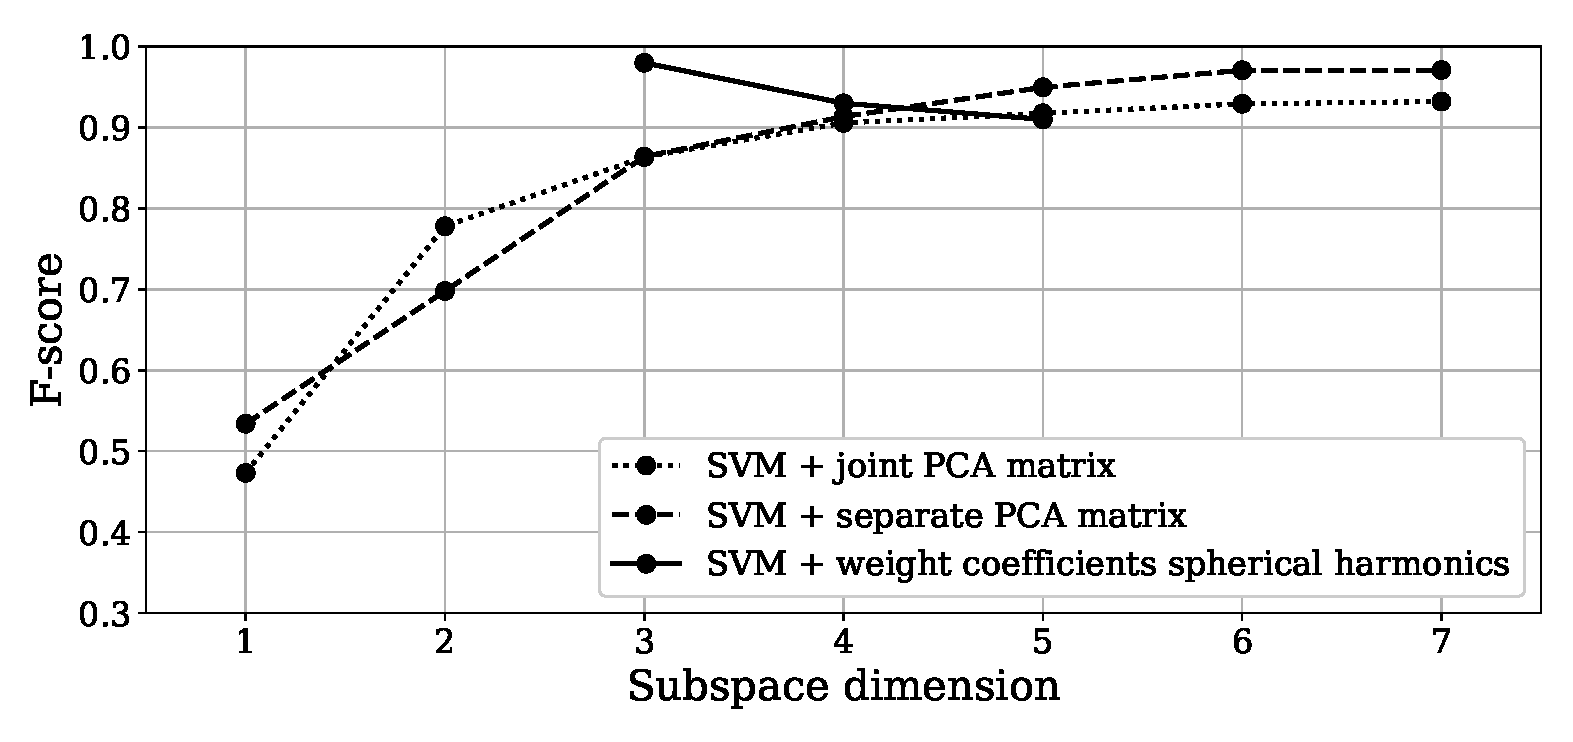
\includegraphics[scale=0.52]{./figs/result_first_eng.eps}
    \caption{Classification F-score on walking, jogging, upstairs for User 1}
    \label{fg:clf_result_one}
\end{figure}
\end{otherlanguage}

The quality of the F-score classification of the movement of one person is shown on Fig.~\ref{fg:clf_result_one}.
It can be seen that three-dimensional spherical harmonics are sufficient for effective classification.
When applying methods trained on the data of the first user to classify time series recorded from the second and third users, the quality decreases depending on the type of movement.
So running and walking are classified better than stair climbing.
The table~\ref{tbl:accuracy_table_all} represents the classification quality for multiple users.
At the same time, due to the increase in the dimension of space, the overall quality of the classification falls. Mean values are shown in Fig.~\ref{fg:clf_result_many} and in the table~\ref{tbl:accuracy_table_mean}.

\begin{otherlanguage}{english}
\begin{table}[H]
    \caption{Mean classification F-score for three users}
    \label{tbl:accuracy_table_mean}
    \centering\medskip\tabcolsep=12pt\small
    \begin{tabular}{l|ccc}
    \hline
        Method & \multicolumn{3}{c}{F-score}\\
    \hline
        Dimension $p$ & 3 & 4 & 5\\
    \hline
        {SVM + weight coefficients spherical harmonics}     & $0.90$ & $0.82$ & $0.81$ \\
        {SVM + joint PCA matrix} & $0.79$ & $0.80$ & $0.89$ \\
        {SVM + separate PCA matrix} & $0.78$ & $0.81$ & $0.81$ \\
    \hline
    \end{tabular}
\end{table}
\end{otherlanguage}

\begin{otherlanguage}{english}
\begin{figure}[H]
    \centering
    \includegraphics[scale=0.52]{./figs/result_mean_eng.eps}
    \caption{Mean and STD F-score for walking, jogging, upstairs}
    \label{fg:clf_result_many}
\end{figure}
\end{otherlanguage}

\begin{otherlanguage}{english}
\begin{table}[H]
\centering
\caption{Comparison table of different movement classes}
\begin{tabular}{p{0.5cm}p{4cm}p{4cm}p{4cm}}
    & Time series segment
    & Phase trajectory
    & Spherical model
    \\
    \hline
    \rotatebox{90}{ \text{Walking} }
    & \includegraphics[scale=0.3]{figs/time_series_wlk_8.eps}
    & 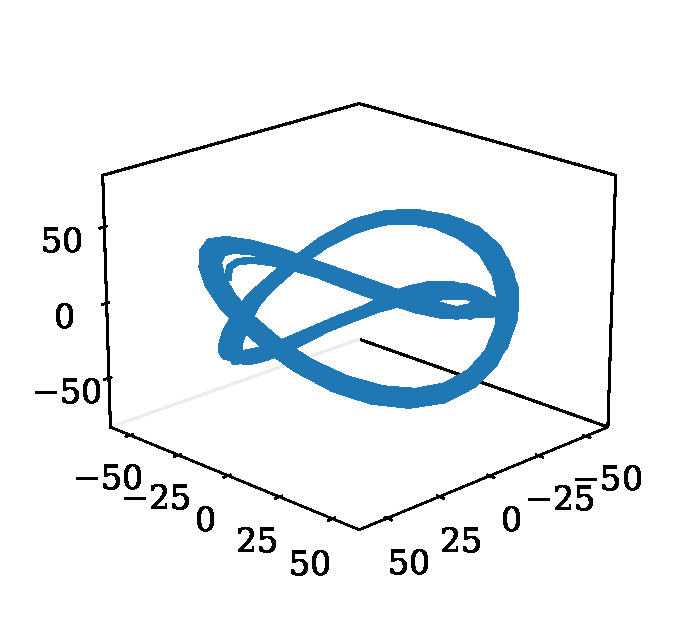
\includegraphics[scale=0.35]{figs/phase_traj_wlk_8.eps}
    & \includegraphics[scale=0.35]{figs/spharm_wlk_8.eps}
    \\ 
    \hline
    \rotatebox{90}{ \text{Jogging} }
    & 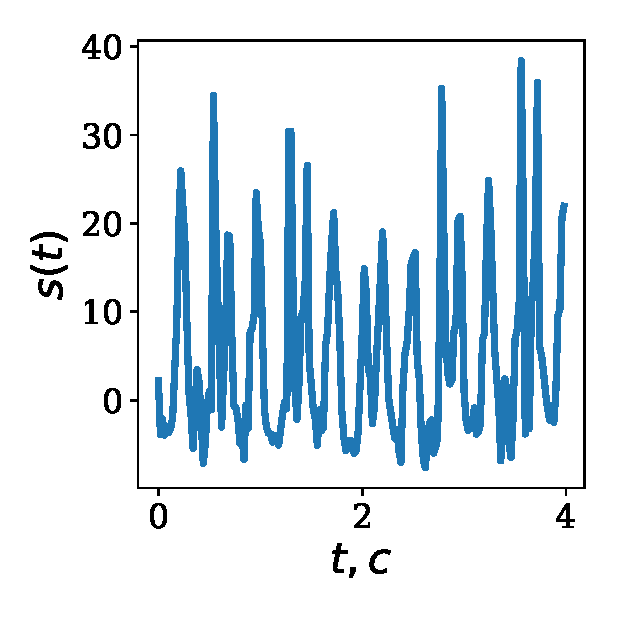
\includegraphics[scale=0.3]{figs/time_series_jog_9.eps}
    & \includegraphics[scale=0.35]{figs/phase_traj_jog_9.eps}
    & \includegraphics[scale=0.35]{figs/spharm_jog_9.eps}
    \\ 
    \hline
    \rotatebox{90}{ \text{Stairs} }
    & \includegraphics[scale=0.3]{./figs/time_series_ups_4.eps}
    & 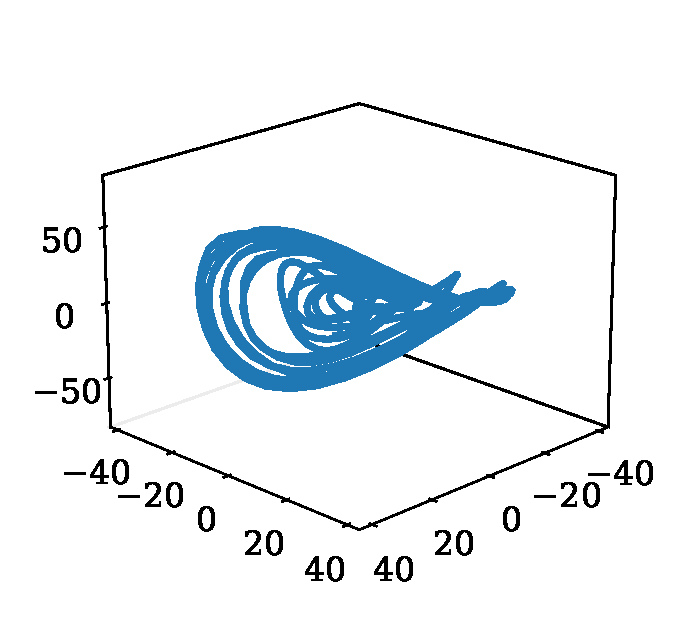
\includegraphics[scale=0.35]{./figs/phase_traj_ups_4.eps}
    & \includegraphics[scale=0.35]{./figs/spharm_ups_4.eps}
    \\ 
    \hline
\end{tabular}
\label{tbl:table_of_figures}
\end{table}
\end{otherlanguage}

The results of the algorithm are shown on table~\ref{tbl:table_of_figures}.
On the left is a fragment of the time series recorded from the accelerometer.
In the center are the obtained phase trajectories in three-dimensional space.
On the right are models of spherical harmonics.
It can be seen that different classes of time series have different trajectories and different approximation models.
%%%%%%%%%%%%%%%%%%%%%%%%%%%%%%%%%%%%%%%%%%%%%%%%%%%%%%%%%%%%%%%%%%%%%%%%%%%%%%%%%%%%%%%%%%
\section{Conclusion}

In the work, the problem of classifying quasi-periodic time series was solved, as well as the problem of constructing a model of the phase trajectory.
To reduce the dimension of the trajectory subspace, the method of principal components was applied to the phase trajectory.
The phase trajectory presented in spherical coordinates was approximated by a linear combination of spherical harmonics.

The experiment was conducted on three time series: accelerometer readings while walking, running and descending stairs for three users with similar height and weight.
The classification quality is high when evaluated on the user on whom the models were trained.
Models of phase trajectories on the surface of a sphere have shown that such an approximation preserves the geometric structure of the sequence of points, and also contains information about the mathematical expectation and dispersion of the phase trajectory.
This is clearly seen in the table~\ref{tbl:table_of_figures} in the figures on the right.
The dark gray area on the surface of the sphere represents the dispersion of the phase trajectory, the black one is the mathematical expectation.
The properties of the approximation model will be separately investigated in future work.
The number of models remains small compared to neural networks or nearest neighbors.
Each stage of the classification has an explicit interpretation.

\newpage
\begin{otherlanguage}{english}
\bibliography{lib}
\end{otherlanguage}
\end{document}
